
%\setcounter{chapter}{-1}


\chapter{Алгоритмы}

\lesson{1}{27.09.2023}{Продолжение}

\section{Продолжение}

% дискретка

\begin{enumerate}
    \item Прибавляем 1 к t
\end{enumerate}

\begin{figure}[H]
    \centering
    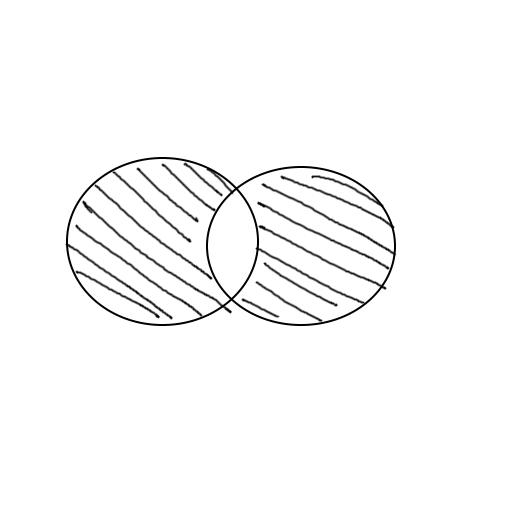
\includegraphics[width=\linewidth]{1.png}
    
    
    \label{fig:1}
\end{figure}

$T_k = M_1 \times M_2 \times \dots \times M_k$

$|M_i| = j$

$(r_1, r_2, \dots, r_k)$

$T_k \leftrightarrow P_k$

\begin{figure}[H]
    \centering
    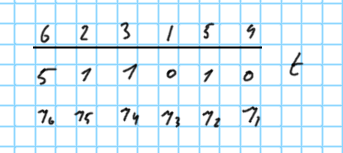
\includegraphics[width=\linewidth]{2.png}
    
    
    \label{fig:2}
\end{figure}

\begin{enumerate}
    \item Прибавляем 1 к t
    \item Определяем номер разряда в котором значение увеличивается на 1, записываем в j
    \item Для любого i от 1 до N такого что i > j, меняем $d_i = -d_i$.
    \item j (не номер, именно такой элемент) меняем с соседом слева если $d_j=-$, и с соседом справа, если $d_j = +$.
\end{enumerate}

\begin{figure}[H]
    \centering
    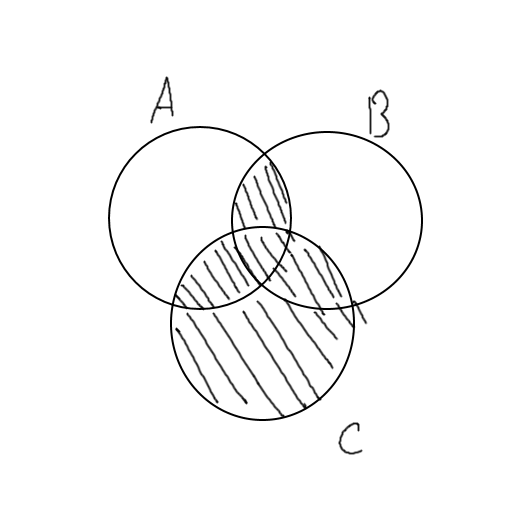
\includegraphics[width=\linewidth]{3.png}
    
    
    \label{fig:3}
\end{figure}

\section{Перебор и нумерации, сочетания}


$C_n^k = \frac{n!}{k!(n-1)!}$

\begin{enumerate}
    \item $C_n^k = C_n^{1-k}$
    \item $C_{n-1}^m + C_{n-1}^{m-1} = C_n^m$ 
\end{enumerate}


$(a + b)^n = \sum_{k = 0}^{n}C_n^k a^k b^{n-k}$


\begin{enumerate}
    \item $a = b = 1$

$2^n = \sum_{k = 0}^{n}C_n^k$

    \item $a = 1$, $b = -1$
    
\end{enumerate}


$(a + b)^n = \sum_{k = 0}^{n}C_n^k a^k b^{n-k}$

$(a + b)^n = (a+b)(a+b)^{n-1} = $
$a(a +b)^{n- 1} + (a + b)^{n - 1} = a \cdot \sum_{k = 0}^{n - 1}C_{n-1}^k a^k b^{n-1-k} +$

$+ b \cdot \sum_{k = 1}^{n-1}C_{n-1}^k a^k b^{n-1-k} = \sum_{k = n}^{n - 1} C_{n-1}^k a^{k + 1} b^{n-1-k} +$

$+ \sum_{k=n}^{n - 1} C_{n-1}^k a^k b^{n-k} = $

$\sum_{k = 1}^{n} C_{n-1}^{k-1} a^k b^{n-k} +$

$+ \sum_{k = 0}^{n - 1} C_{n-1}^k a^k b^{n-k} =$

$= a^n + \sum_{k = 1}^{n - 1} C_{n - 1}^{k-1} a^k b^{n-k} + \sum_{k = 1}^{n - 1} C_{n-1}^k a^k b^{n-k} + b^n$

$= a^n + \sum_{k = 1}^{n - 1}(C_{n-1}^{k-1} + C_{n-1}^k) a^k - b^{n-k} + b^n = $

% Не дописано? на доске конца не нашёл.

\begin{enumerate}
    \item Увеличиваем на 1 номер самого правого элемента который можно увеличить
    \item Справа выписываем натуральный ряд
\end{enumerate}

\begin{figure}[H] % Возможно не отсюда
    \centering
    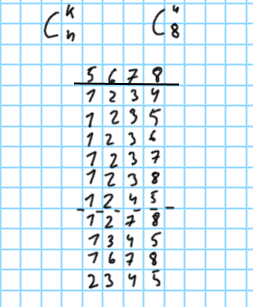
\includegraphics[width=\linewidth]{5.png}
    
    
    \label{fig:5}
\end{figure}

\begin{figure}[H]
    \centering
    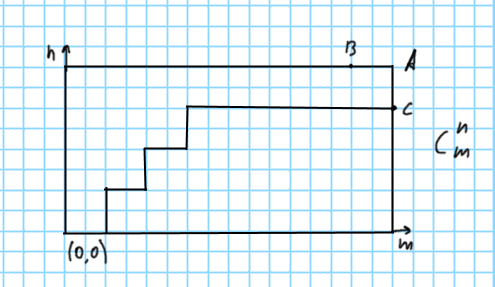
\includegraphics[width=\linewidth]{4.png}
    
    
    \label{fig:4}
\end{figure}

1 3 4 5

(1 0 1 1 1 0 0 0)


$num(b[1:n], m) = \begin{cases}
    num(b[1:n-1], m), b[n] = 0\\
    C_{n-1}^m + num(b[1: n-1], m-1), b[n] = 1\\
\end{cases}$

$num((-1, 0, 1, 0, 1, 0, 1), 4) = C_6^4 + num(b(1,0,1,0,1,0), 3) = C_6^4 + num((1, 0, 1, 0, 1), 3) = C_6^4 + C_4^3 + num((1, 0, 1), 2) = C_4^4 + C_4^3 + C_2^2$



$num((1, ...), 1) = C_6^4 + C_4^3 + C_2^2$

\begin{figure}[H]
    \centering
    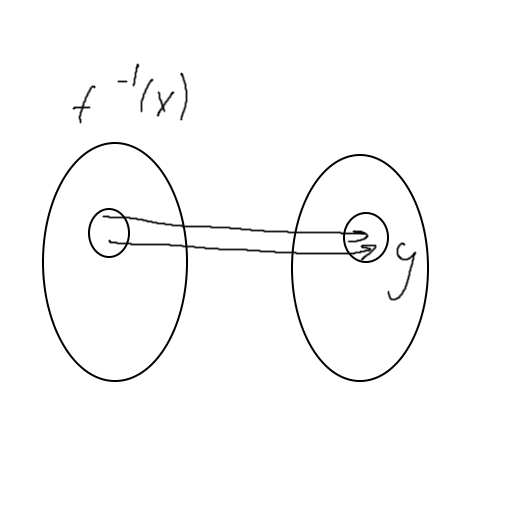
\includegraphics[width=\linewidth]{6.png}
    
    
    \label{fig:6}
\end{figure}




